% Prof. Dr. Ausberto S. Castro Vera
% UENF - CCT - LCMAT - Curso de Ci\^{e}ncia da Computa\c{c}\~{a}o
% Campos, RJ,  2022
% Disciplina: Paradigmas de Linguagens de Programa\c{c}\~{a}o
% Aluno: Rômulo Souza Fernandes


\chapter{Ferramentas existentes e utilizadas}

Neste capítulo será apresentadas algumas ferramentas para auxiliar no desenvolvimento em Python, algumas dessas ferramentas foram utilizadas até mesmo para realizar esse trabalho. A seguir algumas das melhores ferramentas para desenvolvimento utilizando Python.
\begin{itemize}
  \item Nome da ferramenta (compilador-interpretador)
  \item Endere\c{c}o na Internet
  \item Vers\~{a}o atual e utilizada
  \item Descri\c{c}\~{a}o simples (m\'{a}x 2 par\'{a}grafos)
  \item Telas capturadas da ferramenta
  \item Outras informa\c{c}\~{o}es
\end{itemize}

    \section{Notepad++}
	O Notepad++ é um editor de texto de código aberto funcional e gratuito, reconhecendo diversas linguagens de programação, uma delas é o Python. Essa ferramenta também suporta vários idiomas. Sua última versão lançada é a Notepad++ v8.4.7, que está disponível para download gratuitamente no seu site oficial, o link a seguir fará o redirecionamento para a aba de downloads do \href{https://notepad-plus-plus.org/downloads/}{Notepad++}. 
	
	\begin{figure}[H]
		\begin{center}
			\caption{Ambiente de trabalho do Notepad++} \label{ling1}
			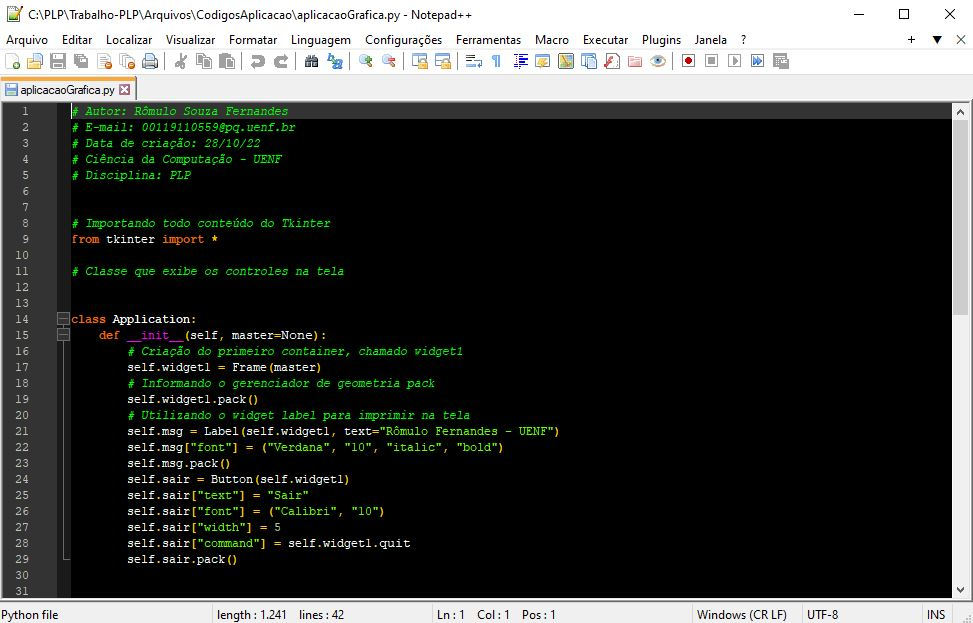
\includegraphics[width=6cm]{notepad.JPG} \\
			{\tiny \sf Fonte:{ Autor}}
		\end{center}
	\end{figure}
	
	Tem a utilização regida pela GNU General Public License. O Notepad++ é escrito em C++ e baseado no Scintilla. Possui alguns recursos muito úteis que são particulares, como a criação de atalhos para chamar programas, agrupa seções de código, permitindo a ocultação de blocos de código, deixando a janela mais legível.
	
    \section{PyCharm}
    O PyCharm é uma IDE especializada em Python desenvolvida pela empresa JetBrains. Oferecendo assim uma ferramenta para desenvolvimento utilizando a linguagem Python. 
    O PyCharm oferta uma grande variedade de ferramentas integradas, como executor teste, depurador, terminal, autocompletamento, ferramentas de banco de dados, controle de versão, terminal SSH, desenvolvimento remoto, integração com Vangrant e Docker.
    Assim permitindo depuração de códigos Python sem exigências externas, incluindo bancos de dados, destaca a sintaxe, verificação em tempo real do código. Além de possuir uma comunidade com suporte ativo. Sua versão paga possibilita o desenvolvimento web, como Flask, Django e Pyramid, além oferecer suporte para XML, CSS, HTML e JavaScript.
    
    De pontos negativos, a ferramenta PyCharm tem um carregamento demorado, necessitando de alguns segundos para abrir por completo. Também necessita de algumas configurações antes de usar certos projetos.
    
    
    \begin{figure}[H]
    	\begin{center}
    		\caption{Ambiente de trabalho do PyCharm} \label{ling1}
    		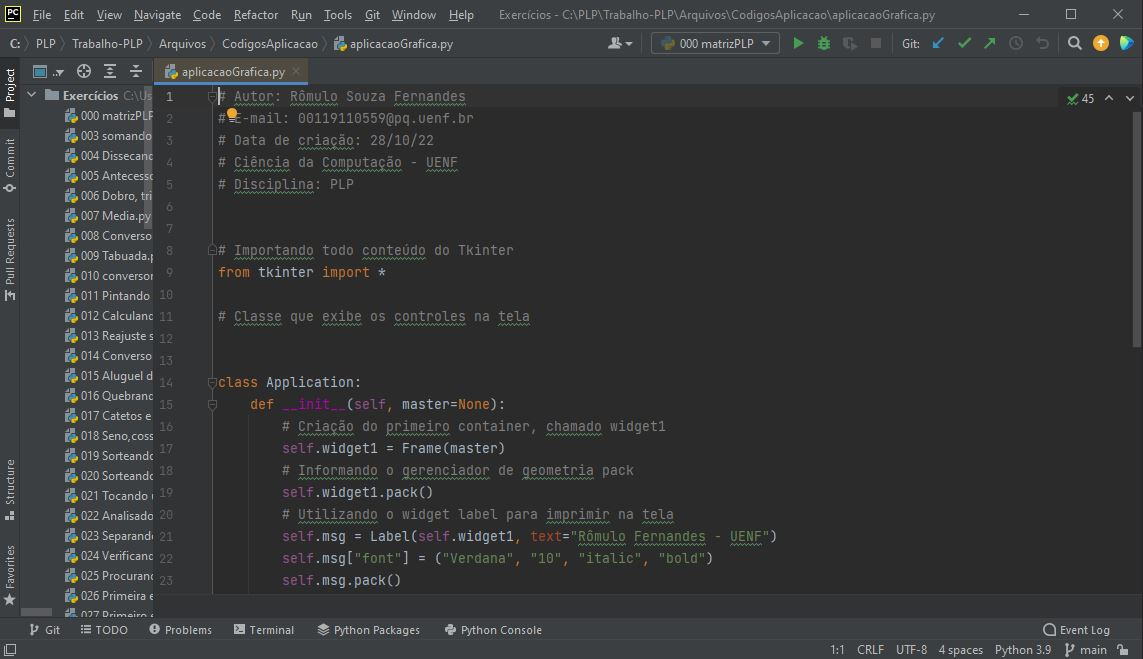
\includegraphics[width=9cm]{pycharm.JPG} \\
    		{\tiny \sf Fonte:{ Autor}}
    	\end{center}
    \end{figure}
    
     A versão utilizada foi a última versão lançada, sendo a 2022.2.4, que está disponível para download no seu site oficial com duas versões, sendo elas a versão Professional com avaliação gratuita por 30 dias e a versão Community, completamente gratuita e com base em open source, o link a seguir fará o redirecionamento para a aba de downloads do \href{https://www.jetbrains.com/pt-br/pycharm/download/#section=windows}{PyCharm}.
    
    \section{Visual Studio Code}
	O Visual Studio Code, também conhecido como VS Code, é uma das IDEs mais populares do mundo, criada pela empresa Microsoft, dando suporte para Windows, Linux e OS. É uma ferramenta para desenvolvimento gratuita e muito completa, permitindo ainda que o usuário faça a adição de extensões, assim acrescentando componentes de acordo com a sua necessidade, contendo em seu total 4700 extensões disponíveis. Essa IDE oferece o preenchimento automático, teste de unidade, depuração, linting, custamização do ambiente de trabalho, oferece também a possibilidade de mudar entre ambientes Python. Além de permitir utilizar o GIT dentro do próprio Visual Studio Code. E uma característica do Visual Studio Code é que o mesmo suporta várias linguagens além do Python.
    
    \begin{figure}[H]
    	\begin{center}
    		\caption{Ambiente de trabalho do VS Code} \label{ling1}
    		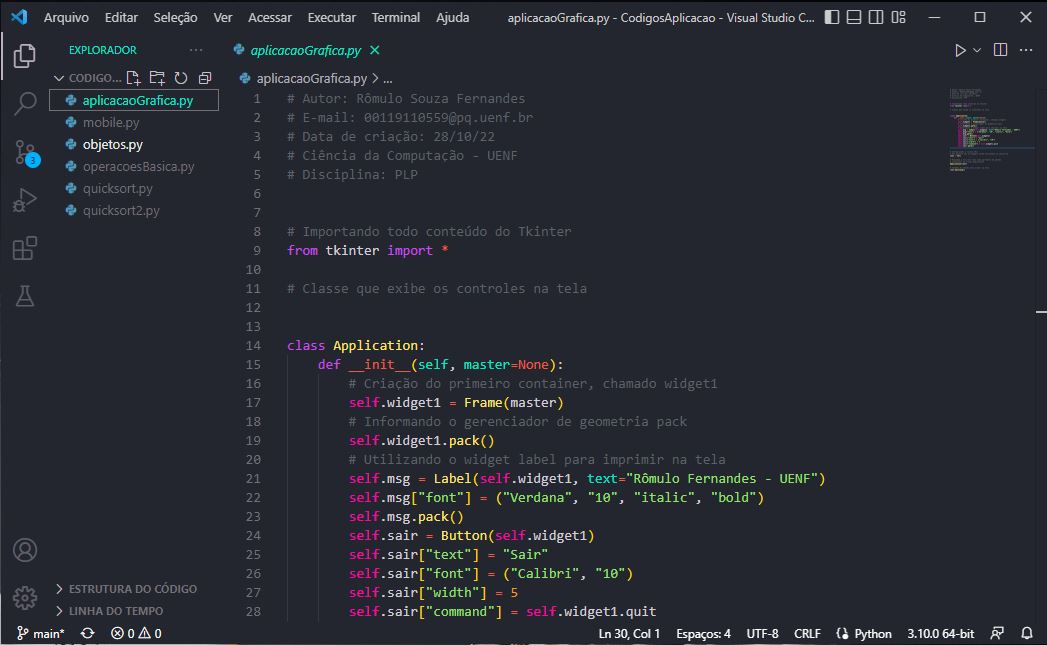
\includegraphics[width=9cm]{vscode.JPG} \\
    		{\tiny \sf Fonte:{ Autor}}
    	\end{center}
    \end{figure}
    
    A versão utilizada foi a última versão lançada, sendo a 1.17.1, que está disponível para download gratuitamente no seu site oficial, o link a seguir fará o redirecionamento para a aba de downloads do \href{https://code.visualstudio.com}{Visual Studio Code}.
    
    \section{Compilador XYZ}


    \section{Interpretador Shell}
	%https://docs.python.org/pt-br/3/tutorial/interpreter.html
	%https://education.ti.com/html/webhelp/EG_TINspire/PT/Subsystems/EG_Python/Content/m_workspaces/ws_shell.HTML

   
    \section{Debug}
     